%%%%%%%%%%%%%%%%%%%%%%%%%%%%%%%%%%%%%%%%%%%%%%%%%%%%%%%%%%%%%%%%%%%%%%%%%%%%%%%%
%2345678901234567890123456789012345678901234567890123456789012345678901234567890
%        1         2         3         4         5         6         7         8

\documentclass[letterpaper, 10 pt, conference]{ieeeconf}  % Comment this line out
                                                          % if you need a4paper
%\documentclass[a4paper, 10pt, conference]{ieeeconf}      % Use this line for a4
                                                          % paper

\IEEEoverridecommandlockouts                              % This command is only
                                                          % needed if you want to
                                                          % use the \thanks command
\overrideIEEEmargins
% See the \addtolength command later in the file to balance the column lengths
% on the last page of the document




% The following packages can be found on http:\\www.ctan.org
\usepackage{graphics} % for pdf, bitmapped graphics files
\usepackage{epsfig} % for postscript graphics files
\usepackage{mathptmx} % assumes new font selection scheme installed
\usepackage{times} % assumes new font selection scheme installed
\usepackage{amsmath} % assumes amsmath package installed
\usepackage{amssymb}  % assumes amsmath package installed
\usepackage{hyperref}
\usepackage{units}
\usepackage{ifthen}
\usepackage{tikz}
\usetikzlibrary{calc}
\usepackage[usenames,dvipsnames]{pstricks}
\usepackage{epsfig}
\usepackage{pst-grad} % For gradients
\usepackage{pst-plot} % For axes
\usepackage[space]{grffile} % For spaces in paths
\usepackage{etoolbox} % For spaces in paths
\makeatletter % For spaces in paths
\patchcmd\Gread@eps{\@inputcheck#1 }{\@inputcheck"#1"\relax}{}{}
\makeatother





\title{\LARGE \bf
Recognition of Fingerspelling in Real-time Video Sequence
}

%\author{ \parbox{3 in}{\centering Huibert Kwakernaak*
%         \thanks{*Use the $\backslash$thanks command to put information here}\\
%         Faculty of Electrical Engineering, Mathematics and Computer Science\\
%         University of Twente\\
%         7500 AE Enschede, The Netherlands\\
%         {\tt\small h.kwakernaak@autsubmit.com}}
%         \hspace*{ 0.5 in}
%         \parbox{3 in}{ \centering Pradeep Misra**
%         \thanks{**The footnote marks may be inserted manually}\\
%        Department of Electrical Engineering \\
%         Wright State University\\
%         Dayton, OH 45435, USA\\
%         {\tt\small pmisra@cs.wright.edu}}
%}

\author{Aniket Dhar$^{1}$ and Philipp Duernay$^{2}$% <-this % stops a space
\thanks{$^{1}$Aniket Dhar PUT STUDENTNO}%
\thanks{$^{2}$Philipp Duernay - 4622227 - p.durnay@student.tudelft.nl}%
}




\begin{document}



\maketitle
\thispagestyle{empty}
\pagestyle{empty}


%%%%%%%%%%%%%%%%%%%%%%%%%%%%%%%%%%%%%%%%%%%%%%%%%%%%%%%%%%%%%%%%%%%%%%%%%%%%%%%%
\begin{abstract}

TODO

\end{abstract}


%%%%%%%%%%%%%%%%%%%%%%%%%%%%%%%%%%%%%%%%%%%%%%%%%%%%%%%%%%%%%%%%%%%%%%%%%%%%%%%%
\section{INTRODUCTION}

The accuracy of modern computer vision systems enables a wide range of applications for computers to support society, not only in our daily-life activities, but also in health care or even safety-critical situations. Detection of diseases, cruise control and pedestrian detection are only a few examples to name. 

In this project we explore another possible application for computer vision: the recognition of sign language. As a final goal one can image a smartphone app which translates sign language in real-time enabling a normal conversation between deaf and hearing people.

As a first start in that direction we start by recognizing the fingerspelling alphabet as shown in \autoref{fig:abc}. We implement and evaluate a computer vision system that can detect the static gestures of this alphabet\footnote{Letter J and Z involve movement and are not part of this project} in a video sequence in real-time. 

\begin{figure}[hb]
\centering
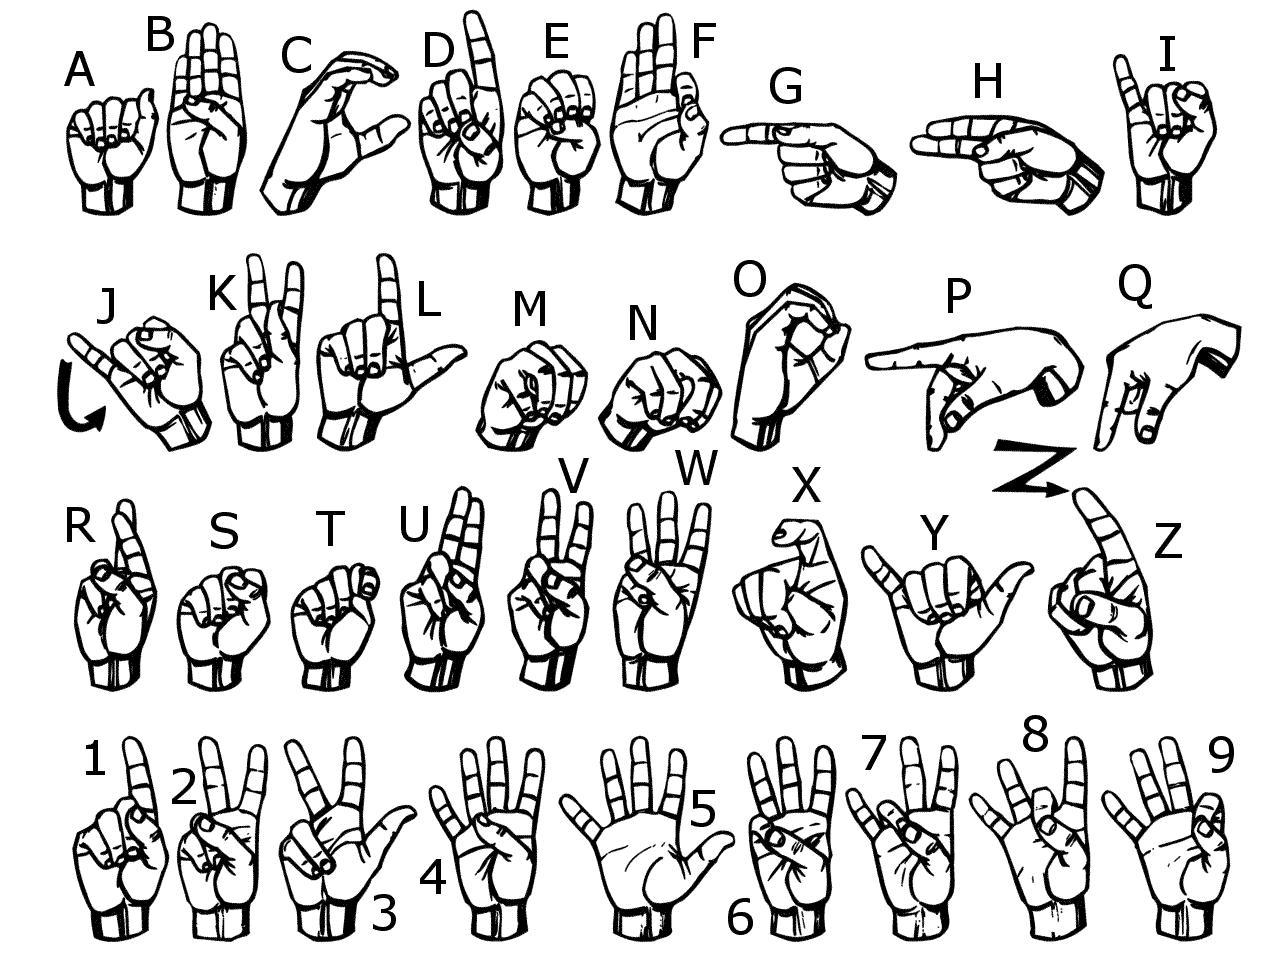
\includegraphics[width=0.8\linewidth]{abc.png}
\caption{American Fingerspelling Alphabet}
\label{fig:abc}
\end{figure}

For that we build a classification system and train it on a dataset of static images. As a proof of concept we embed the obtained model in a small application. The application reads a video stream from the webcam, segments the hand of the user and shows the recognized letter.

For computer vision applications one can make use of a lot of tools and libraries that are already implemented. In this project we use \textit{python3} together with \textit{OpenCV} and some other libraries. A full overview is given in \autoref{sec:appendix} 

The project has been carried out in context of the Computer Vision course at Delft University of Technology. This report describes the work flow of our project, the applied methods as well as the obtained results.TODO one sentence results

The remaining parts or this document are structured as follows: \autoref{sec:appr} describes our approach and the implemented methods. \autoref{sec:eval} contains an evaluation of the implemented methods and the respective results. \autoref{sec:concl} concludes the project and gives a short look ahead.


\section{Approach}
\label{sec:appr}
The aim of the project is to recognize letters from the sign alphabet in a video sequence. To achieve this we take a classical supervised learning approach: we learn a model from labeled examples off-line, then we apply the trained model on video frames.

We identify three main ingredients that are required for the final application: (1) Object descriptors that represent the pose of the hand unambiguously, (2) a model that we can train on a dataset with labeled descriptors, (3) an application that extracts the hand descriptors from a video sequence and matches it with the trained model.

For all steps we tried different approaches. These are described in further detail in the following sections. 

\subsection{Training Data}

In total we found two sets that are suitable for our purpose, namely a set from University of Exeter\footnote{\url{http://empslocal.ex.ac.uk/people/staff/np331/index.php?section=FingerSpellingDataset}} and a set from Thomas Moeslund's\footnote{\url{http://www-prima.inrialpes.fr/FGnet/data/12-MoeslundGesture/database.html}}. For the rest of the document we refer to the first one as the \textit{ASL-set} and the second one as the \textit{TM-set}.

The TM-set contains between 50-100 black and white images per class for the 24 letters of the alphabet. The subjects wear a black sweater and the pictures are taken in front of a black background. An example can be seen in \autoref{fig:tm-set}.

The lightning conditions should make the segmentation quite easy, as there is a big contrast between the hand and the background. However, the lightning conditions are also quite artificial and do not resemble a natural use case. Thus it is questionable whether a model trained on that dataset can perform well in a real application.

The ASL-Set contains 2500 coloured images per class for the 24 letters of the alphabet, taken from 5 different subjects. The pictures have been taken from a kinect camera with more or less equal lightning conditions. An example can be seen in \autoref{fig:asl-set}. Next to the image also depth data is available which can be used for segmentation.

The pictures contain strong shadows and a lot of time the face of the user is also visible on the picture. Although this resembles much more our final use case, it makes colour-based segmentation much harder. The depth data can help in segmentation on the dataset, but we can't rely on it in the final use case, as it is not available for our webcam.

\begin{figure}
\centering
\begin{minipage}{0.4\linewidth}
	\centering
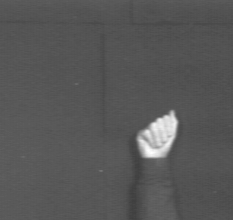
\includegraphics[height=3cm]{a-tm}
\caption{Example image for the TM-set}
\label{fig:tm-set}
\end{minipage}
\hfill
\begin{minipage}{0.4\linewidth}
	\centering
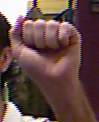
\includegraphics[height=3cm]{a-asl}
\caption{Example image for the ASL-set}
\label{fig:asl-set}
\end{minipage}
\end{figure}
\subsection{Segmentation}

For our project we want to separate the hand from the image background. As the shape of the hand can be different in every image we can't use shape-based features for segmentation. Instead we try several texture-based approaches.

Segmentation can also be seen as a two class classification problem. Given a pixel we are looking for the probability that it belongs to the hand or to the background. Based on that probability we can assign it to one of the two. More formally this would be:

\begin{equation}
	\textbf{assign } y_1 \textbf{ to x if } p(y_1|x) > p(y_0|x \textbf{ else } y_0
\end{equation}
With $y_1$ as label for the hand and $y_0$ as label for the background. 

\subsection{Colour Threshold}

The most straight-forward way is to to use a colour range for segmentation. For example a gray threshold or the a skin colour range. As long as the lightning conditions are good and no other objects with the same color are on the image, it can already work reasonably well. 

For this approach we define the likelihood of a pixel being part of the hand:

\begin{equation}
p(y_1 | x) = \begin{cases}
1 & \quad \text{if } \gamma_1 < x < \gamma_2 \\
0 & \quad \text{otherwise}
\end{cases}
\end{equation}
With $\gamma$ as the threshold(s).

This approach can easily be implemented using conditioned indexing with numpy arrays. All pixels of an image that contain a colour value that is higher than a certain threshold are copied to a new image.

We evaluate a gray value threshold on the TM-set, where everything else but the hand is quite dark. An example can be seen in \autoref{fig:tm-segment}, where we cropped the hand of the part with the highest probability. Here we already get satisfying results.

\begin{figure}
	\centering
	\begin{minipage}{0.4\linewidth}
		\centering
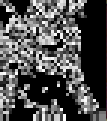
\includegraphics[height=3cm]{asl-hist-segment}
\caption{Likelihood for colour-histogram segmentation on ASL-set}
\label{fig:asl-hist-segment}
	\end{minipage}
	\hfill
	\begin{minipage}{0.4\linewidth}
		\centering
		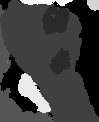
\includegraphics[height=3cm]{asl-depth}
		\caption{Depth data int the ASL-set}
		\label{fig:asl-depth}
	\end{minipage}
\end{figure}


On the ASL-set we try skin-color-based segmentation. We set a range of TODO in HSV colour space to be part of the hand and everything else to be background.

TODO put example

\subsubsection{Colour Histogram}

A colour histogram consists of a histogram for every colour channel. The histogram can be calculated for a range of pixels and therefore capture a colour distribution over several pixels. Thus it is more reliable than a simple colour threshold.

In our approach we first calculate an average histogram for hand pixels, then we define the class conditional probability as the difference to that average histogram. Inspired by the last lab session we define the likelihood as:

\begin{equation}
p(y_1 | x) = e^{-\frac{d(\bar{\phi},\phi(x))}{\sigma}}
\label{eq:hist}
\end{equation}
Where $\phi$ denotes the histogram function, \textbf{d} denotes the KL divergence and $\sigma$ is a scaling factor.

Also this approach can be implemented with numpy arrays. The calculation of the KL divergence we integrate from them MATLAB script of the last lab session to python.

On the ASL-set the hand is in almost all cases in the center of the picture. Thus we can obtain the average histogram taking the average histogram for a 6-by-6 window in the center of the picture across the whole dataset. Then we can apply \autoref{eq:hist} with a 6-by-6 sliding window over every image. An example can be seen in \autoref{fig:asl-hist-segment}, where the likelihood is represented in intensity values.

\begin{figure}
\centering
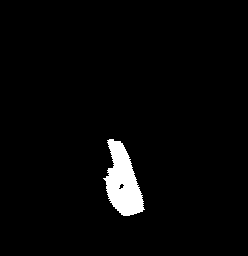
\includegraphics[height=3cm]{tm-segment}
\label{fig:tm-segment}
\caption{Colour-threshold segmentation on TM-set}
\end{figure}

The example shows the likelihood for \autoref{fig:asl-set} one can easily see that the results are not satisfactory. Although big parts of the background are seperated properly, the method fails on image parts where the colour is similar to skin colour. This can be seen in at the face of the subject, as well as the yellow background. Another problem is the big differences even on the hand. All together we don't consider this approach as promising enough.

\subsubsection{Background Subtraction}

Background subtraction [TODO REF] is a way to separate fore- and background in videos. A background frame is calculated and subtracted from the current frame. Thus only objects that changed their appearance remain in the dissimilarity image.

As our application will only run on a stationary webcam, we can assume that the hand is the only moving object and background subtraction is applicable. However, the approach can't be applied during training, where we only have static images available.

For the calculation of the background frame we take an average across several frames. We define a likelihood model for background subtraction as follows:

\begin{equation}
p(y_1 | x) = e^{-\frac{||\bar{x}-x||)}{\sigma}}
\label{eq:backg}
\end{equation}
Where $\bar{x}$ is the background, and $\sigma$ a scaling factor.

We implement this using the OpenCV API. Next some bluring we use \texttt{accumulatedSum()} to calculate the average image and \texttt{absdiff()} to subtract the background.

An example for a described dissimilarity image can be seen in \autoref{fig:bg-subtr}. The method looks promising as the hand is clearly separable. However, if we move the hand slowly, or the lightning conditions are bad big parts of the hand are also taken as background.

\begin{figure}
	\centering
	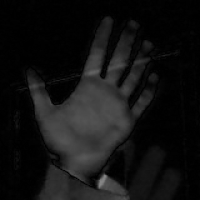
\includegraphics[height=3cm]{bg-subtr}
	\label{fig:tm-segment}
	\caption{Dissimilarity image for background subtraction}
\end{figure}

\subsubsection{Depth Segmentation}

For the ASL-set depth data is available. An example can be seen in \autoref{fig:asl-depth}, where the depth data for \autoref{fig:asl-set} is displayed in grayscale. The low resolution of the data is apperant as only about 5 different levels are visible. Although it enables us to separate the background partly, for most pictures it is not enough to segment the hand entirely. However, we can use the method in combination with other segmentation methods.

We measure the depth at the center of the image and take it as baseline. Then we calculate the likelihood as follows:

\begin{equation}
p(y_1 | x) = e^{-\frac{||x_{center}-x||)}{\sigma}}
\label{eq:backg}
\end{equation}
Where $x_ {center}$ is depth value at the center of the image, and $\sigma$ a scaling factor.

Also here the implementation is quite straight forward. The image is stored in a similar way as a grayscale image. Thus we can subtract the depth value of the center from the whole image and obtain the distance matrix. 

\subsubsection{Nearest Neighbour Classifier}

Instead of just measuring values on the image we can also train a classifier on labeled examples. As we want to do the segmentation for the video in real-time, we need a classifier that can be trained quickly. This makes the knn-classifier a good choice.

Labeled examples are unfortunately not available in the given data set, so we use a hands-on method to obtain those. Similar to the histogram method we sample a window of 6-by-6 pixels in the picture center as objects with label $y_1$. Additionally we can use depth segmentation or background subtraction to obtain background samples with label $y_0$. 

Once the classifier is trained it can be used to label the whole image. As we did not implement the classifier ourselves we don't go into detail about its functionality here and refer to standard pattern recognition literature.

For the implementation we use the 3-nearest-neighbour implementation from \texttt{sklearn}. The library allows training a model and obtaining predictions.

\subsubsection{Markov Random Field}

A Markov Random Field (MRF) [TODO REF] enables the incorporation of spatial conditions with label probabilities. We use it to combine these spatial conditions with several of the methods described before.

We apply the depth segmentation and background subtraction model to get soft labels for back and foreground. Additionally we train the knn-classifier as described and obtain another set of soft labels for the image. Then we can define the combined likelihood as a weighted sum of the score of the nearest neighbour classifier and of the background calculation. This can be formulated as follows:
\begin{equation}
p(y_1 | x) = \alpha * s_{knn}(_1 | x) + \beta * s_{backgr}(x_1 | x) 
\end{equation}
With $\alpha$ and $\beta$ as weights and $s_{knn}$ and $s_backgr$ as the respective soft labels.

For defining spatial structures we take the image gradient. We want the edge value to drop when there was an edge in the initial image. Therefore we assign edges on y and x axis with the respective gradients $I_y, I_x$ multiplied by -1.

In total this gives us the following Markov Random Field:
\begin{center}

%\psscalebox{0.8 0.7} % Change this value to rescale the drawing.
{
\begin{pspicture}(0,-4.2)(5.285984,4.2)
\label{fig:mrf-graph}
\psellipse[linecolor=black, linewidth=0.04, dimen=outer](2.6,3.6)(0.6,0.6)
\psellipse[linecolor=black, linewidth=0.04, dimen=outer](0.6,0.04)(0.6,0.6)
\psellipse[linecolor=black, linewidth=0.04, dimen=outer](4.6921678,0.06)(0.5938165,0.58)
\psellipse[linecolor=black, linewidth=0.04, dimen=outer](2.7,-3.64)(0.58,0.56)
\psellipse[linecolor=black, linewidth=0.04, dimen=outer](2.64,0.12)(0.6,0.6)
\psellipse[linecolor=black, linewidth=0.04, dimen=outer](3.82,1.24)(0.58,0.56)
\psellipse[linecolor=black, linewidth=0.04, dimen=outer](1.54,-1.08)(0.6,0.6)
\psline[linecolor=black, linewidth=0.04, arrowsize=0.05291667cm 2.0,arrowlength=1.4,arrowinset=0.0]{<-}(0.82689905,0.7149105)(2.24,3.16)
\psline[linecolor=black, linewidth=0.04](1.1875665,0.023503793)(2.0924335,0.056496207)
\psline[linecolor=black, linewidth=0.04](3.0637367,0.4422136)(3.7362633,1.1177864)
\psline[linecolor=black, linewidth=0.04](3.2675664,0.023503793)(4.1724334,0.056496207)
\psline[linecolor=black, linewidth=0.04](1.9037366,-0.6777864)(2.5762634,-0.0022135878)
\psline[linecolor=black, linewidth=0.04, arrowsize=0.05291667cm 2.0,arrowlength=1.4,arrowinset=0.0]{<-}(2.6,0.76)(2.56,3.04)
\psline[linecolor=black, linewidth=0.04, arrowsize=0.05291667cm 2.0,arrowlength=1.4,arrowinset=0.0]{<-}(1.626899,-0.44508946)(2.36,3.04)
\psline[linecolor=black, linewidth=0.04, arrowsize=0.05291667cm 2.0,arrowlength=1.4,arrowinset=0.0]{<-}(3.52,1.72)(2.88,3.04)
\psline[linecolor=black, linewidth=0.04, arrowsize=0.05291667cm 2.0,arrowlength=1.4,arrowinset=0.0]{<-}(4.48,0.8)(3.040533,3.1537228)
\psline[linecolor=black, linewidth=0.04](0.72,-0.64)(0.92,-0.96)
\psline[linecolor=black, linewidth=0.04, arrowsize=0.05291667cm 2.0,arrowlength=1.4,arrowinset=0.0]{->}(1.8270663,-1.6564572)(2.48,-3.16)
\psline[linecolor=black, linewidth=0.04, arrowsize=0.05291667cm 2.0,arrowlength=1.4,arrowinset=0.0]{->}(2.6596117,-0.5451615)(2.68,-3.04)
\psline[linecolor=black, linewidth=0.04, arrowsize=0.05291667cm 2.0,arrowlength=1.4,arrowinset=0.0]{->}(4.3823037,-0.5819679)(3.08,-3.12)
\psline[linecolor=black, linewidth=0.04, arrowsize=0.05291667cm 2.0,arrowlength=1.4,arrowinset=0.0]{->}(3.6670663,0.62354285)(2.88,-3.08)
\psline[linecolor=black, linewidth=0.04, arrowsize=0.05291667cm 2.0,arrowlength=1.4,arrowinset=0.0]{->}(1.44,-1.76)(2.28,-3.28)
\rput[bl](3.44,2.64){$p(y_1|x)$}
\rput[bl](3.68,-2.4){$p(y_0|x)$}
\rput[bl](2.48,3.44){$y_1$}
\rput[bl](2.6,-3.8){$y_0$}
\rput[bl](4.56,-0.04){$x_2$}
\rput[bl](1.4,-1.2){$x_3$}
\rput[bl](0.48,-0.08){$x_0$}
\rput[bl](2.56,0.0){$x_1$}
\rput[bl](3.72,1.12){$x_4$}
\rput[bl](3.6,-0.28){$-I_x$}
\rput[bl](2.04,-0.84){$-I_y$}
\rput[bl](1.16,0.2){$-I_x$}
\rput[bl](2.72,0.64){$-I_y$}
\end{pspicture}
}


\end{center}

This way we incorporate information of spatial structures like edges and corners, colour information as well as movement/depth information in our model. The final labelling we obtain with the maxflow graph cut algorithm.

For the implementation we use the \texttt{maxflow} package for python. The package allows us to define a graph and to assign weights according to \autoref{fig:mrf-graph}. After that we can execute the maxflow algorithm and obtain the labeled image. The first result still contains some noise. Therefore we apply several bluring/eroding and closing operations, using OpenCV, to obtain a cleaner result.

An example for the method can be seen in \autoref{fig:mrf-example} and \autoref{fig:mrf-example-video}. The results look quite promising and in this first evaluation we consider it as our best method so far.

\begin{figure}
	\centering
	\begin{minipage}{0.4\linewidth}
		\centering
		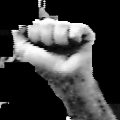
\includegraphics[height=3cm]{mrf}
		\label{fig:mrf-example}
		\caption{Segmentation with Markov Random Field on ASL-set}
	\end{minipage}
	\hfill
	\begin{minipage}{0.4\linewidth}
		\centering
		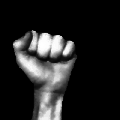
\includegraphics[height=3cm]{mrf-video}
		\label{fig:mrf-example-video}
		\caption{Video Segmentation with Markov Random Field}
	\end{minipage}
\end{figure}


\subsection{Representation}

Once the hand is properly segmented from the background we need to define descriptors for the hand shape that enable an accurate recognition. As we are interested in the shape of the hand, shape based descriptors seem to be a reasonable approach at first. However, also these need to be obtained from the image. In several letters it is particular necessary to also capture the shape of the fingers inside the hand and not only the overall shape. In the ASL-set and on the video there are a lot of shadows in the pictures which make this not an easy task.

Therefore we mainly worked on region-based descriptors. The approaches are described in the following.

\subsubsection{Grayscale-Pixel}

This can be seen as one of the most straight-forward representation. We convert the segmented image to a grayscale image, vectorize it and obtain the feature vector.

The drawback of the method is that less important features not particularly filtered, which results in a huge feature vector. These are generally harder to classify (Curse of dimensionality). Additionally the representation is not rotation/scale invariant.

\subsubsection{Edge-Pixel}

A lot of information about the shape is contained in the edges. If we are able to detect the important edges, we can take the contours of the hand as a shape representation. Therefore we apply the Canny edge detection algorithm [TODO REF] to obtain a binary image with the most important edges. These binary images are vectorized and used as feature vectors.

This method still leads to a high feature vector and is similar to the grayscale pixel approach not rotation/scale invariant.

\subsubsection{Histogram of Gradients}

HoG-features [TODO REF] are commonly used for object detection. The image gradient is calculated for the whole image. Then in a fixed window size a histogram is formed containing the distribution of image gradients.

These features incorporate change in intensity value and should therefore be more informative than the simple Edge-Pixel representation. Especially because the slight changes in shape of the fingers on the hand can be detected.

However, the same drawback as described in the previous paragraphs holds. The representation is not rotation/scale invariant.

In contrast to the first two methods we need our own implementation for HoG-features. We use OpenCV to obtain the image gradients, subsequently we calcualate the angular and magnitude using numpy functions.

\subsubsection{Bag of HoGs}

To compensate for the rotation invariance we apply a "Bag-of-" method. Here we apply a KMeans clustering to obtain the most common histograms of the ASL-dataset. Then we represent Each object by the distance to this codebook. Inspired by MILES [TODO REF] we calculate the distance as follows:

\begin{equation}
	\phi(x) = min\{ e^{||x-x_{codebook}||}\}
\end{equation}

Thus the distance of a image to a code word is defined by the distance of its closest instance. The measure should give a high similarity if the HoGs of two objects are similar even if they are at different places in the image.

This method basically builds upon the previous method. After having obtained the HoG-features for all images we use KMeans clustering from the sklearn library to get the codebook.

\subsubsection{Principal Component Analysis}

A general way to deal with high dimensionality or less informative features is principal component analysis [TODO REF]. Here we transform the feature space by keeping the maximal variance. We evaluate PCA on top of the previously described methods. The principal components are chosen in a way that 90\% of the variance is kept.

Also here we use the sklearn library. It provides as with functions to scale the data, as well as to apply PCA.

\subsection{Classification}

After having segmented the image and transformed it to a representation we can train a classifier. The focus of the work was on the preceeding steps, which is why we only evaluate several standard classifiers. These are:

\begin{itemize}
	\item Nearest Neighbour, because it can be trained quickly 
	\item Linear Support Vector Machine, because it can cope with large feature dimensions
	\item Neural Network, because it generally performs well
\end{itemize}

In the video the user will not change the shown letter every couple of milliseconds. Thus we have several frames per sample available and can exploit that for classification. 

We take a sequence of 5 frames per sample and classify each. The final prediction is based on a majority vote. Additionally we can set a "confidence" threshold to avoid misclassification. If not at least 75 \% of the predictions are the same, we reject the classification and a "Letter not recognized" is displayed on the screen.

The majority voting we implement ourselves. The classifiers are taken from sklearn library.

\section{Evaluation}
\label{sec:eval}
We select several combinations among the methods described in the previous chapters for evaluation. In a first step we evaluate the methods on the two datasets in cross-evaluation. The methods with the best results, we train on the whole dataset and evaluate in the video.

\subsection{Performance on Datasets}

We set up a 6-folded cross-evaluation for all methods where we measure the mean performance in accuracy and its standard derivation. An overview of the evaluated methods and their results is given in \autoref{tab:eval-methods}

\begin{table}[h]
\caption{Evaluated methods}
\label{tab:eval-methods}
\begin{center}
\begin{tabular}{c|c|c|c|c}
Dataset & Segmentation & Representation & Classifier & Accuracy \\
\hline
\hline
TM-set & Gray-thresh & Edge-Pixel & SVM &\\
TM-set & Gray-thresh & HoG & SVM &\\
ASL-set & MRF & HoG & SVM &\\
ASL-set & MRF & Bag of HoGs & SVM & \\
\hline
\end{tabular}
\end{center}
\end{table}

TODO blabla results

TODO put confusion matrix

\subsection{Performance on Video}

For the video evaluation two subjects try every letter and .. TODO

\begin{table}[h]
\caption{Evaluated methods}
\label{tab:eval-methods}
\begin{center}
\begin{tabular}{c|c|c|c|c}
Trainingset & Segmentation & Representation & Classifier & Accuracy \\
\hline
\hline
TM-set & MRF & HoG & SVM &\\
ASL-set & MRF & HoG & SVM &\\
\hline
\end{tabular}
\end{center}
\end{table}

TODO bla bla

TODO put confusion matrix for best one

\begin{table*}[h]
\caption{Confusion Matrix}
\label{table_example}
\begin{center}
\begin{tabular}{|c|c|c|c|c|c|c|c|c|c|c|c|c|c|c|c|c|c|c|c|c|c|c|c|c|}
\hline
 &A & B & C & D & E & F & G & H & I &K&L&M&N&O&P&Q&R&S&T&U&V&W&X&Y\\
\hline
A &  &  &  &  &  &  &  &  & & & & & & & & & & & & & & &  \\
\hline
B &  &  &  &  &  &  &  &  & & & & & & & & & & & & & & &  \\
\hline
C &  &  &  &  &  &  &  &  & & & & & & & & & & & & & & &  \\
\hline
D &  &  &  &  &  &  &  &  & & & & & & & & & & & & & & &  \\
\hline
E &  &  &  &  &  &  &  &  & & & & & & & & & & & & & & &  \\
\hline
F &  &  &  &  &  &  &  &  & & & & & & & & & & & & & & &  \\
\hline
G &  &  &  &  &  &  &  &  & & & & & & & & & & & & & & &  \\
\hline
H &  &  &  &  &  &  &  &  & & & & & & & & & & & & & & &  \\
\hline
I &  &  &  &  &  &  &  &  & & & & & & & & & & & & & & &  \\
\hline
K &  &  &  &  &  &  &  &  & & & & & & & & & & & & & & &  \\
\hline
L &  &  &  &  &  &  &  &  & & & & & & & & & & & & & & &  \\
\hline
M &  &  &  &  &  &  &  &  & & & & & & & & & & & & & & &  \\
\hline
N &  &  &  &  &  &  &  &  & & & & & & & & & & & & & & &  \\
\hline
O &  &  &  &  &  &  &  &  & & & & & & & & & & & & & & &  \\
\hline
P &  &  &  &  &  &  &  &  & & & & & & & & & & & & & & &  \\
\hline
Q &  &  &  &  &  &  &  &  & & & & & & & & & & & & & & &  \\
\hline
R &  &  &  &  &  &  &  &  & & & & & & & & & & & & & & &  \\
\hline
S &  &  &  &  &  &  &  &  & & & & & & & & & & & & & & &  \\
\hline
T &  &  &  &  &  &  &  &  & & & & & & & & & & & & & & &  \\
\hline
U &  &  &  &  &  &  &  &  & & & & & & & & & & & & & & &  \\
\hline
V &  &  &  &  &  &  &  &  & & & & & & & & & & & & & & &  \\
\hline
W &  &  &  &  &  &  &  &  & & & & & & & & & & & & & & &  \\
\hline
X &  &  &  &  &  &  &  &  & & & & & & & & & & & & & & &  \\
\hline
Y &  &  &  &  &  &  &  &  & & & & & & & & & & & & & & &  \\
\hline
\end{tabular}
\end{center}
\end{table*}


\section{CONCLUSIONS}
\label{sec:concl}
TODO

\addtolength{\textheight}{-12cm}   % This command serves to balance the column lengths
                                  % on the last page of the document manually. It shortens
                                  % the textheight of the last page by a suitable amount.
                                  % This command does not take effect until the next page
                                  % so it should come on the page before the last. Make
                                  % sure that you do not shorten the textheight too much.

%%%%%%%%%%%%%%%%%%%%%%%%%%%%%%%%%%%%%%%%%%%%%%%%%%%%%%%%%%%%%%%%%%%%%%%%%%%%%%%%



%%%%%%%%%%%%%%%%%%%%%%%%%%%%%%%%%%%%%%%%%%%%%%%%%%%%%%%%%%%%%%%%%%%%%%%%%%%%%%%%



%%%%%%%%%%%%%%%%%%%%%%%%%%%%%%%%%%%%%%%%%%%%%%%%%%%%%%%%%%%%%%%%%%%%%%%%%%%%%%%%
\section*{APPENDIX}
\label{sec:appendix}
\subsection{Implementation}
TODO used libraries
TODO what did we implement
TODO put link to code




\end{document}
